\chapter[Verification of Analytical Expression of GFT]{Verification of Analytical Expression of GFT for Optical Cavities}\label{App:analyticalGF}
In this part, we will examine the Lorentz form of GFT with exact numerical calculations on a H3 PC cavity, a micropillar cavity and homogeneous medium. As shown later, if CPU time increases, the numerical calculation results approach the analytical expression (error $\leq 5\%$). The numerical calculation error is $\leq 2\%$ as shown in the homogeneous test. Notice that the H3 PC cavity mode is a typical cavity with highly confined cavity mode, and the micropillar cavity has a typical smooth mode field distribution. Both cavities should have represented the commonly used cavities. That is to say, one can safely use the Lorentz approximation for bare cavity GFT calculations.

One bonus of this approximation is that one can obtain the bare cavity GFTs at any place just with a quick computation using a mode monitor on the cavity, rather than a very hard computation using multi time monitors, if using Lumerical Solutions to calculate the cavity mode.

Note that some plots in this Appendix have tiny labels. Since I cannot re-plot the figures at present, I will describe the important observations in the captions, instead.

\section{$\mathbf{G}^{A}$ and $\mathbf{G}^{Num}$}
There are two ways to obtain the bare cavity GFTs. One is fully based on numerical calculation of the mode dynamics at source and detector positions by distributing time monitors in FDTD simulation using Lumerical Solutions. Since we cannot write down the explicit expression for the GFT in this calculation approach, we call the GFTs obtained through this approach as numerical GFTs or notate them as $\mathbf{G}^{Num}$. The calculation theory is presented in Section~\ref{section:GFT}.
We can notate the numerical GFT calculated in FDTD method as  \[\mathbf{G}^{Num}=\mathbf{G}^{FDTD}.\]

The other approach is to use the Lorentz approximation introduced in Section~\ref{section:Lorentz} and to substitute the field strength into a Lorentzian function to gain the bare cavity GFTs between any two points. Although this approach also calls for a numerical calculation on the cavity mode or field, the GFTs we get can be expressed in explicit formulas. Therefore, we call the GFTs obtained in this approach analytical GFTs, or label them as $\mathbf{G}^{A}$. In this approach, we only need a 2-D or 3-D mode monitor in Lumerical Solutions to calculate the bare cavity GFTs, which calls for less computation memory and CPU time. Therefore, we often use the analytical approach for GFT calculations.

So far, there is no publication addressing whether these two methods are equivalent. In principle, they should be equivalent, as both of the approaches assume the emission source is a dipole, which has a Lorentzian function of oscillation. To some extent, the term ``Lorentz approximation'' used here is also a dipole approximation. Before we move on the detailed GFT calculations, let us double check the equivalence of these two methods and estimate the error of our calculations in these two approaches.



Further notice that a general Green function should include two parts: one is cavity mode GF, which comes from the cavity mode; the other is radiative GF, which includes evanescence, leaky mode and homogeneous radiation contributions. If written in a formula, the total Green function for a typical optical cavity is
\begin{equation}
 \label{Ganal}
\mathbf{G}^{Total}=\mathbf{G}_{cav}+\mathbf{G}_{rad},
\end{equation}
where $\mathbf{G}_{cav}$ is the cavity field contribution, and $\mathbf{G}_{rad}$ is the radiative contribution. The radiative Green function for an effective slab of microcavity usually has no approximated explicit expression.
As we have calculated using an effective three-layer slab model, which is commonly used for PC cavity cases, the evanescent contribution part is negligible in the total GFT, once the distance of dipoles is large enough (larger than $20$ nm if in a Si slab). And the homogeneous contribution is usually less than 0.1\% of $G^{total}$ (see Fig.\ref{Ghom_11_12_13}). The leaky mode contribution is small too, for a high-Q cavity. Hence, at least in the high-Q PC cavity cases presented in this thesis, we can safely use
\begin{equation}
 \label{GanalandGcav}
\mathbf{G}^{Total} \approx \mathbf{G}_{cav}.
\end{equation}
For more accurate calculations, one can use $G^{rad} \approx G_{hom}$ if the evanescent and leaky mode contributions are negligible.

The total Green function of a cavity can be calculated numerically (see Appendix~\ref{App:FDTD_GFT}), which implies that
\begin{equation}
\mathbf{G}^{Num} = \mathbf{G}_{Total}.
\end{equation}
Therefore, this chapter of appendix is to examine if we can use the analytical GF to approximate the total GF in the cases of PC cavity and micropillar cavity to be studied in Chapter~\ref{ch:cavity}, and in general cavity cases presented in Chapter~\ref{ch:ensemble}.

The analytical bare cavity Green function reads (the theoretical deviation can be referenced in PP37-39 of \cite{Sakoda2005})
\begin{equation}
 \label{Gcav}
\mathbf{G}^{A}_{cav}(\br,\br',\omega)
=\sum_{c\lambda}{\frac{\omega^2\mathbf{f}_{c\lambda}(\mathbf{r},\omega_{c\lambda})\mathbf{f}_{c\lambda}^*(\mathbf{r}',\omega_{c\lambda})}
{\omega_{c\lambda}^2-\omega^2-i\omega\Gamma_{c\lambda}}},
\end{equation}
with $c\lambda$ denoting modes of the cavity, $\Gamma_{c\lambda}$ the decay rate or FWHM of $\mathbf{f}_{c\lambda}(\omega)$ for the corresponding mode.

Among equations above, mode frequency $\omega_{c\lambda}$ can be read from a FDTD run with a broadband dipole source,
and we have the following relations:
\begin{subequations}
\begin{align}
  {}& \quad \quad \quad \quad \quad \quad \mathbf{f}_{c\lambda}(\mathbf{r},\omega_{c\lambda})\mathbf{f}_{c\lambda}^*(\mathbf{r}',\omega_{c\lambda})
= \mathbf{f}_{c\lambda}(\mathbf{r},\omega_{c\lambda}) \otimes \mathbf{f}_{c\lambda}^*(\mathbf{r}',\omega_{c\lambda}),\\
=& \! \left( \! \begin{array}{c}
               f_{c\lambda}^x(\mathbf{r},\omega_{c\lambda})f_{c\lambda}^{x*}(\mathbf{r}',\omega_{c\lambda}) \quad
                 f_{c\lambda}^x(\mathbf{r},\omega_{c\lambda})f_{c\lambda}^{y*}(\mathbf{r}',\omega_{c\lambda}) \quad
                 f_{c\lambda}^x(\mathbf{r},\omega_{c\lambda})f_{c\lambda}^{z*}(\mathbf{r}',\omega_{c\lambda}) \\
               f_{c\lambda}^y(\mathbf{r},\omega_{c\lambda}){f}_{c\lambda}^{x*}(\mathbf{r}',\omega_{c\lambda}) \quad
                 f_{c\lambda}^y(\mathbf{r},\omega_{c\lambda}){f}_{c\lambda}^{y*}(\mathbf{r}',\omega_{c\lambda}) \quad
                 f_{c\lambda}^y(\mathbf{r},\omega_{c\lambda}){f}_{c\lambda}^{z*}(\mathbf{r}',\omega_{c\lambda}) \\
               f_{c\lambda}^z(\mathbf{r},\omega_{c\lambda}){f}_{c\lambda}^{x*}(\mathbf{r}',\omega_{c\lambda}) \quad
                 f_{c\lambda}^z(\mathbf{r},\omega_{c\lambda}){f}_{c\lambda}^{y*}(\mathbf{r}',\omega_{c\lambda}) \quad
                 f_{c\lambda}^z(\mathbf{r},\omega_{c\lambda}){f}_{c\lambda}^{z*}(\mathbf{r}',\omega_{c\lambda})
              \end{array} \! \right) \! \label{fmatrix},
\end{align}
\end{subequations}
\begin{align}
|\mathbf{f}_{c\lambda}(\mathbf{r}_{antinode},\omega_{c\lambda})|^2 &{} \approx  \frac{1}{{\rm V}_{eff}\varepsilon(\mathbf{r}_{antinode})},\label{EVeff}\quad \\
{\rm Q} &= \frac{\omega_{c\lambda}}{\Gamma_{c\lambda}}\label{Q},
\end{align}
where $\Gamma_{c\lambda}$ and ${\rm Q}$ can be obtained via Harminv,
and $\mathbf{r}_{antinode}$ is the position in a cavity where the field strength has the maximum amplitude. Notice that I have used a Matlab version of Harminv developed by Mark Patterson in my study, but there is also an open source version in MIT's Ab-Initio physics website (http://ab-initio.mit.edu/wiki/index.php/Harminv).

The typical steps to calculate $\mathbf{G}^{A}_{cav}$ can be generalized as follows:

\textbf{Step 1}: Run FDTD calculation with a broadband dipole source
and a point time monitor. A frequency monitor is also recommended to be used, which is broadband and has dense data collecting points.

Note that placing the dipole source in the symmetric center can save the CPU time, since we can employ symmetric boundary conditions in this case.
If the dipole is in a high symmetric point, however, some modes may be forbidden, and a frequency monitor possibly cannot detect some modes.
In this sense, a ``blind'' run using a point time monitor with a dipole source both at non-symmetric centers is necessary before detailed calculation.
For the discussions below, the default FDTD calculation environment is Lumerical FDTD Solutions V6.5 or above~\cite{LumericalSolutions}, and the default monitor used is a point time monitor.

\textbf{Step 2}: Calculate the cavity parameters by analyzing the data collected by the time monitors.

If this is the first time to run the FDTD calculation with the dipole source setting introduced in step 1,
read out the modes' resonant frequency or resonances through a broadband frequency monitor in FDTD software.
Compare the observations of wave envelopes obtained from the time monitors to identify if the field dynamic curve is far from converging to a straight line. Then run the simulation again with improved settings, such as elongated running time, until the wave envelopes detected by the time monitors are all close to zero or a straight line (reference to the $\mathbf{E}(t)$ plots in Figs. \ref{Gmp30_combine} and \ref{G69_combine}). The field evolution data from the time monitors can be extracted to Harminv to obtain the resonant frequencies $\omega_{c\lambda}$, and hence decay rates $\Gamma_{c\lambda}$ and $Q$ factor from Equ.\eqref{Q}.

Notice that a time monitor gives all three components of E-field. One can only calculate one set of cavity parameters in one polarized direction per run in Harminv. Sometimes, one may need to discard a part of initial data or some E-field data in certain polarization directions. Which part of data should be deposed depends on the source setting and the property of the cavity. For instance, an $x$-polarized electrical dipole source may not be able to excite an E-field in $y$-direction in some PC cavity; therefore, the $y$-component of the detected E-field data for this cavity should not be used to calculate the cavity parameters, even though there may be some non-zero $y$-polarized E-field data collected in the time monitors.
Usually, to get all three components of the GFTs using E-field data of a cavity, one may need to run the simulation three times by orientating the dipole source in one of the three orthogonal directions per run.

%Now, extract the detected time-domain E-field (e.g. the $x$-component) into, for example, time.dat file.
% by running
%\begin{center}
%\begin{tabular}{c}
%\begin{lstlisting}[framexrightmargin=-4cm]
%load  data.mat
%% write the Ex into time.dat file row by row
%dlmwrite('time.dat', time_Ex, 'delimiter', '\n', 'precision_for_data_step', '%.12f');
%\end{lstlisting}
%\end{tabular}
%\end{center}
%in Matlab.
%Now, you may need to discard part of the record where mixed with the strong dipole source signal,
%and only remain the mode signal in the time.dat file. Possibly, there are some fast or slow oscillations
%(noises, perhaps caused by the reflection from the PML boundaries) in the detected wave envelopee,
%we may also want to filter them out. And the other components or detected data from other positions may give a better results.
%So, it's better to view the detected wave envelopee and only collect meaningful signals into time.dat file.


%Then in terminal, run Harminv command in the same directory
%to read the ${\rm Q}$ factors, resonant frequencies $\omega_{c\lambda}$ and hence decay rates $\Gamma_{c\lambda}$ from Equ. (\ref{Q}).
%\lstset{language={C}}
%\begin{center}
%\begin{tabular}{c}
%\begin{lstlisting}[framexrightmargin=-5cm]
%harminv -t [dt] [lower_freq_border-upper_freq_border] <time.dat >scanQ.log
%\end{lstlisting}
%\end{tabular}
%\end{center}
%where parameter ``dt'' means time step, which can be read from Matlab;
%``lower\_freq\_border'' and ``upper\_freq\_border'' are the two limits of interested freqency range, respectively.
%Results will be written into a file. Reading the file, we can get the required quantities,
%including the peak frequency of ${\rm Q}$.
%This can also be done by running harmiv.m function in Matlab.


\textbf{Step 3}: Improve the data quality by optimizing the simulation settings. Detailed operations are as follows.

Narrow down the dipole bandwidth around one interested mode frequency $\omega_{c\lambda}$ and set required time monitors in place,
re-run the FDTD calculation and get the mode or field data. Now, we need both time monitors (to get $\mathbf{G}^{FDTD}$ in interested points, ${\rm Q}$ factor,
as well as other related quantities) and frequency monitors (to get the modes and $\mathbf{G}^{A}_{cav}$).
We can add the different types of monitors one by one in several rounds of FDTD runs. Many trial runs may be helpful to find the best simulation settings. As mentioned before, to get all tensor elements of cavity GFTs, one may need to run the simulation three times. In each run, the spots to be placed with monitors should be either the sources or detectors positions for the GFT calculation next.

%For the time monitors, we only put them in some interested positions and make sure the dipole source in the right place ($\mathbf{r}_n$).


The frequency monitors can be set to monitor an area (2D) or a volume (3D) in several discrete frequencies.
Since this global monitor may cost a huge amount of memory and CPU time,
one needs to carefully select a few, not too many, frequency points to monitor.
%However, a global frequency monitor (even reduced to a lower dimension) is needed to calculate the effective mode volume.
What's more, if the dipole sources bring in considerable noises to our concerned mode,
one needs to trigger off the frequency monitor after the dipole source's strong oscillating.

One also needs a global index monitor to get the index distribution data of the cavity. The data can be collected by solely running a quick simulation
(run the simulation and quickly exit the simulation before the mode calculation begins), or by running a separated simulation only with an index monitor.

If one has a powerful computer cluster or workstation,
one can submit and run many simulation tasks simultaneously,
each of which only has one type of monitors to save time,
and to reduce the data package size.
%And this can also reduce the memory usage and the volume of output file--which is significant,
%because we can hardly handle a big data package in our personal computer when we have to handle them once we want to analyze them.

\textbf{Step 4}: Repeat {\bf Step 2} and further narrow down frequency range of the dipole source to get a good data set of ${\rm Q}$, $\omega_{c\lambda}$, and $\Gamma_{c\lambda}$ for specified mode.
Now, one can compute the $\mathbf{G}^{FDTD}$, by plugging the data collected from the time monitor into Equ. (\ref{def:GFT}).

\textbf{Step 5}: Based on the data collected by the index and frequency monitor,
one normalizes the cavity modes $c\lambda$ by applying Equ. (\ref{normf}),
and gets the effective mode volume ${\rm V}_{eff}$ by applying
\begin{equation}
 \label{normf}
\mathbf{f}_\lambda(\mathbf{r})=\mathbf{f}_\lambda^0(\mathbf{r})/V_{eff}=\frac{\mathbf{f}_\lambda^{FDTD}(\mathbf{r})}{F_\lambda^{antinode}V_{eff}},
\end{equation}
\begin{equation}
 \mathbf{V}_{eff}=\mathbf{V}=\int_V \! \mathrm{d}\mathbf{r} \, \varepsilon(\mathbf{r})(\mathbf{f}^0_\lambda(\mathbf{r}))^* \cdot \mathbf{f}^0_{\lambda'}(\mathbf{r}).
\end{equation}
Please see Appendix~\ref{section:schema4bareGFT} for the detailed normalization process.

%The Matlab code below can be used to do so:
%%\begin{minipage}{160.62\fullwidth}\hcentre
%\lstset{language={Matlab}}
%%\begin{table}\label{normalization}
%%\caption{Normalization of field}
%\begin{center}
%\begin{tabular}{c}
%\begin{lstlisting}[framexrightmargin=-3.5cm]
%% Start getting mode voluems and ensure that modes are properly normalized
%% First normalize to maximum values
%phix = abs(Ex).^2;
%phiy = abs(Ey).^2;
%phiz = abs(Ez).^2;
%phi1 = ((abs(Ex).^2).*epsx+(abs(Ey).^2).*epsy+(abs(Ez).^2).*epsz);
   % epsx=squeeze(index_index_x(:,:,:)).^2 and etc.
%phi2 = max(max(max(phi1)));
%phixr = phix./phi2;
%phiyr = phiy./phi2;
%phizr = phiz./phi2;

%% now get V_eff and normalize with respect to mode Volume
%dv = dx*dy*dz; % or in 2D case dv = dx*dy;
%Veff = sum(sum(sum(phixr.*epsx+ phiyr.*epsy + phizr.*epsz)))*dv;

%Ex = Ex./sqrt(phi2)./sqrt(Veff);
%Ey = Ey./sqrt(phi2)./sqrt(Veff);
%Ez = Ez./sqrt(phi2)./sqrt(Veff);
%% check: sum(sum(sum(abs(Ex).^2.*epsx+abs(Ey).^2.*epsy+abs(Ez).^2.*epsz)))*dv
%clear phix phix0 phiy phiy0 phiz phiz0 phixr phiyr phizr
%\end{lstlisting}
%\end{tabular}
%\end{center}
%%\end{table}
%%\end{minipage}

\textbf{Step 6}: Substitute the parameters gotten above into Eqs.~\ref{fmatrix} and~\ref{Gcav} to calculate all elements of the $\mathbf{G}^{A}_{cav}$ tensor.


%This double-run scheme also suits for calculating $\mathbf{G}^{FDTD}$, using Eq. (\ref{def:GFT}).
%The only difference is that we have to set the monitor time long enough so to perform a precisive Fourier transformation.

Now, one can compare $\mathbf{G}^{A}_{cav}$ and $\mathbf{G}^{FDTD}$.
%we can estimate the value of $\mathbf{G}^{A}_{rad}$, which may contribute to the inhomogeneous broadenning of total PL potentially.
If $\mathbf{G}^{A}_{cav}$ is approximately equal to $\mathbf{G}^{FDTD}$,
we can confidently accept the analytical GFTs as the total GFTs.
%by only employing the frequency and index monitors, to do further calculation
%without bothering ourselves to setup time monitors point by point and run for a long time.


Note that the GFs (no matter whether numerical or analytical) we calculated in this appendix chapter refer to the bare cavity GFs. In the presence of $N$-dipoles, the total GFs should be calculated using the method introduced in Section~\ref{section:GN} by combining the bare cavity GFs and emitter contributions together.

Below, we will present our calculation results on the comparison of $\mathbf{G}^{A}$ and $\mathbf{G}^{Num}$, and error estimation, and present a technique to reduce FDTD simulation burden using symmetric settings.



%%%%%%%%%%%%%%%%%%%%%%%%%%%%%%%%%%%%%%
% This part is to verify Gnum and Ga in a homogeneous medium, from Ganal.tex

\section{The Equivalence of $\mathbf{G}^{A}$ and $\mathbf{G}^{Num}$}\label{section:verifyGAGN}

This section reports a comparison between $\mathbf{G}^{A}$ and $\mathbf{G}^{Num}$ in the cases of Micropillar cavity~\cite{Reitzenstein2007} and PC cavity~\cite{Akahane2003}. It turns out that $\mathbf{G}^{Num}$ and $\mathbf{G}^{A}$ match up very well, once the running time is long enough. In the next section, we will present the factors that may cause some computational errors, and estimate the computational error of GFs.

Calculation results for Micropillar and PC cavities are shown in Figs.~\ref{Gmp30_combine} and~\ref{G69_combine}. The GFs plots show that the analytical and numerical GFs agree very well.

The final result is good enough. However, before obtaining a good result, there were some differences between analytical GFs ($G^{A}$) and numerical ones ($G^{Num}$), either in their amplitudes (or scales) or in their peak positions (may approach 0.01THz in some calculations). I will present some trials in the course of reducing the calculation errors in the next three sections. The factors discussed in the following sections may be only a part of possible factors which can affect the calculation errors. Other factors can also affect the computation accuracy significantly for specific cases. I would like to leave the question open, and report what I did and found in my trials.

\begin{figure}[H]
\centering
\begin{center}
{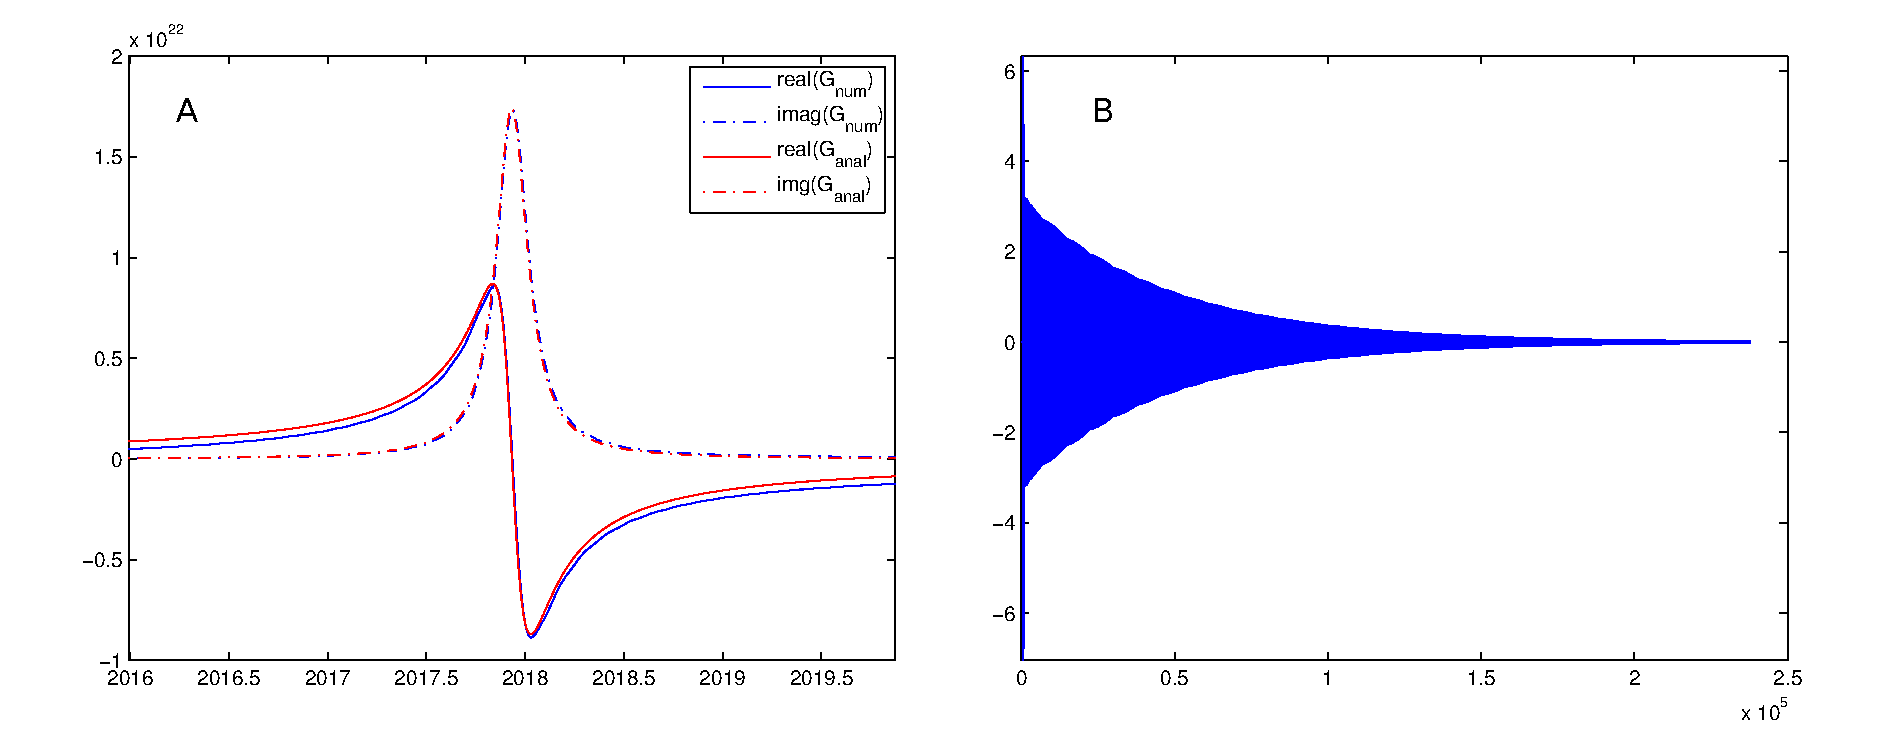
\includegraphics[width=16cm]{./Figs/Gmp30_combine}}
\end{center}
\caption[GF for a micropillar laser.]{\textbf{  $\mathbf{G}^{A}$ (red) and $\mathbf{G}^{Num}$ (blue) comparison for a Micropillar cavity. (A)} $G^{A}(r_1,r_1,\omega)$ and $G^{Num}(r_1,r_1,\omega)$ (I have subtracted $G^{hom}$ (contributes less than 0.1\%) from the original $G^{num}$) in a Micropillar reported in Ref.~\cite{Reitzenstein2007}. The x-axis is frequency in the unit of THz. The y-axis is the amplitude of GFs in an arbitrary unit. $\Gamma$ is read from Harminv. And I have set $\omega_0/2\pi=321.164\,$THz. \textbf{(B)} E field at $r_1$ as a function of simulated time (long enough to do a good FFT). The x-axis is time in the unit of fs. The y-axis is the amplitude of E-field strength in an arbitrary unit.}
\label{Gmp30_combine}
\end{figure}

\begin{figure}[H]
\centering
\begin{center}
{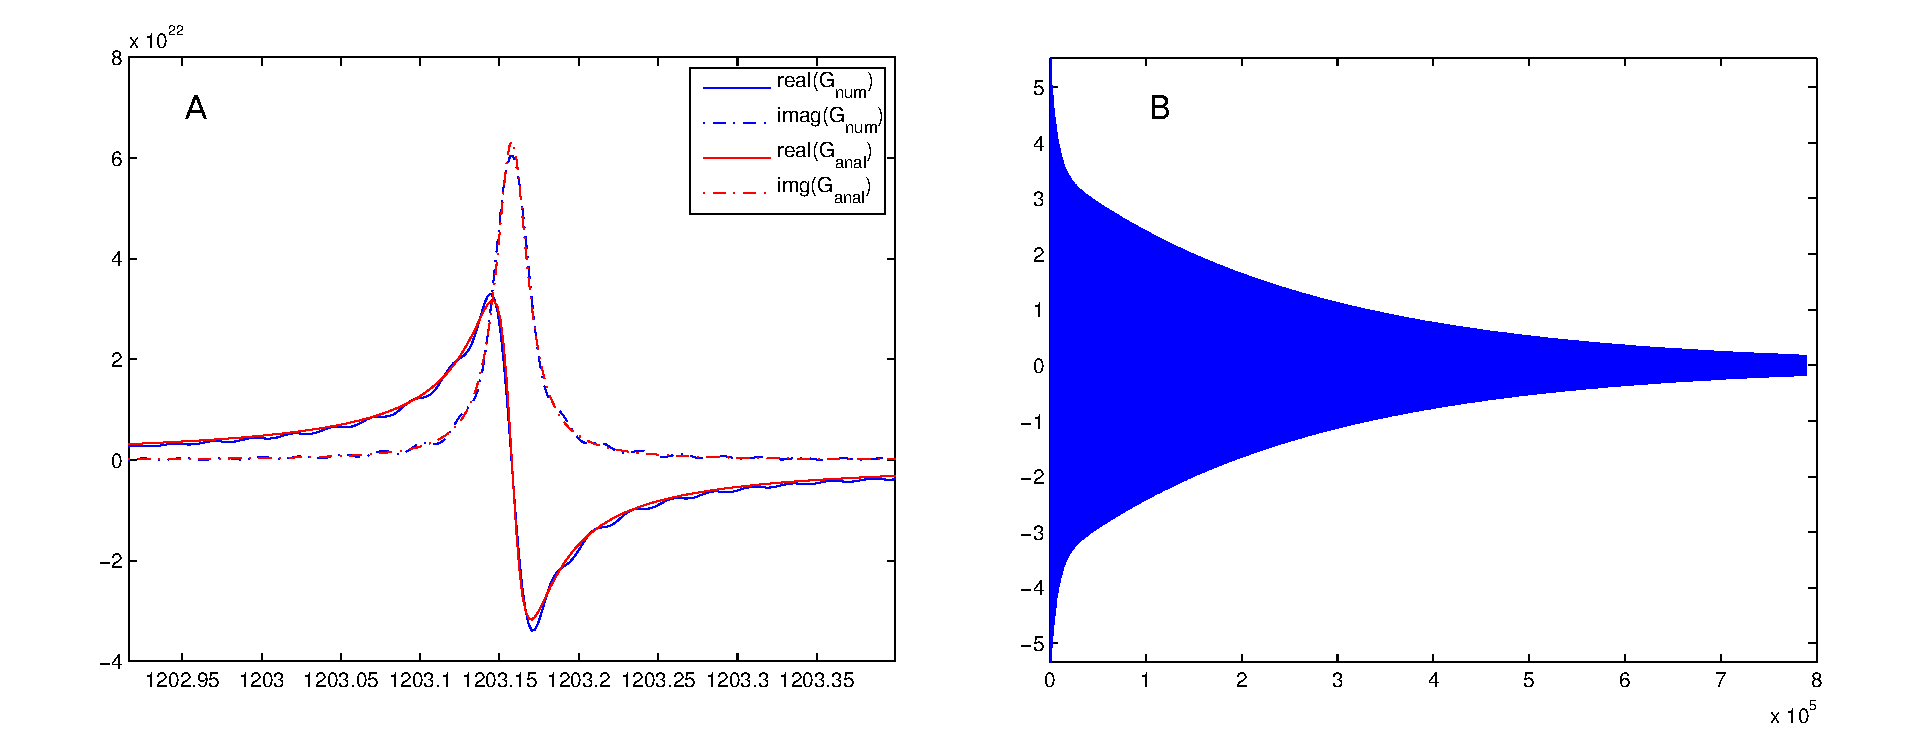
\includegraphics[width=16cm]{./Figs/G69_combine}}
\end{center}
\caption[GF for a PC cavity.]{\textbf{  $\mathbf{G}^{A}$ (red) and $\mathbf{G}^{Num}$ (blue) comparison for a PC cavity. (A)} $G^{A}(r_1,r_1,\omega)$ and $G^{Num}(r_1,r_1,\omega)$ (I have subtracted $G^{hom}$ (contributes less than 0.1\%) from the original $G^{Num}$) in a H3 PC cavity~\cite{Akahane2003}. $\Gamma$ is read from the Harminv. And I have set $\omega_0/2\pi=191.4885\,$THz. \textbf{(B)} E field at $r_1$ as a function of simulated time. The small fluctuations in subfig.~(A) mainly results from the simulation time, which is not long enough to do a good FFT. The coordination notations for both plots are the same as Fig.~\ref{Gmp30_combine}.}
\label{G69_combine}
\end{figure}


%\maketitle


%\maketitle
%\subsection{Results and Discussion}
%In this section, I will basically following the verification steps discussed in the previous section, and discuss the results.
\section{Improving the Accuracy of $\mathbf{G}^{Num}$ Calculation}\label{section:homcheck}
The most significant factor which can make the $\mathbf{G}^{Num}$ inaccurate is the simulation time. Limited simulation time can broaden the envelope of $\mathbf{G}^{Num}$, and bring in some fluctuations in the curves, and decrease the peak value of GFs (see Fig.~\ref{Gpc_errors}(B)). To increase the accuracy of $\mathbf{G}^{Num}$, it is important to elongate the running time and make the field oscillation converge to zero. Related parameter settings, such as reflection rate of PML, can affect the computational accuracy as well. The mechanisms of most setting parameters are straightforward, but how the interpolation setting works in FDTD Solutions is obscure. I will present a discussion on interpolation settings in detail as follows.

To get how much the interpolation settings contribute to the computational error, I run FDTD simulation in homogeneous medium with different interpolation method settings and calculated the GFs. I used silicon (the PC's material) as the homogeneous medium, and made the simulation settings basically the same as that of full simulation in the PC cavity configuration we have discussed in the other sections. The mesh grid is $20\, nm \times 17.3205\, nm \times 21\, nm$. I used a time monitor to calculate $G_{yy}$ at the dipole source, which locates at the origin. In the Lumerical's interpolation setting, there are two different options: one is ``none'' interpolation, the other is to ``nearest mesh cell''. They are different approaches to read out the data from FDTD calculation in Lumerical, by interpolating the discrete data on calculated Yee cell points in different ways (see Lumerical's support website). If considering the interpolation methods in post-coding process, we have several possible calculation approaches to examine, based on FDTD algorithm.

One calculation approach is as follows. We use ``none'' interpolation in Lumerical, and place two time monitors in the half way of two Yee cell (mesh grid) points in x-axis, and respectively on the left and right side of the origin (our interested point with a dipole source); after the FDTD simulation, we interpolate or average the data of two-monitor measurements to get the value at the origin point. We can call this calculation approach the many-joint-monitor approach. For this simulation, I placed the dipole at the origin, and one time monitor at (10, 0, 0) nm, the other time monitor at (-10, 0, 0) nm. The results are shown in Fig.~\ref{Ghom_11_12_13} (A,B and C). The $G^{A}$ in the plots is the analytical function of homogeneous GF.
\begin{figure}[htp]
\centering
\begin{center}
{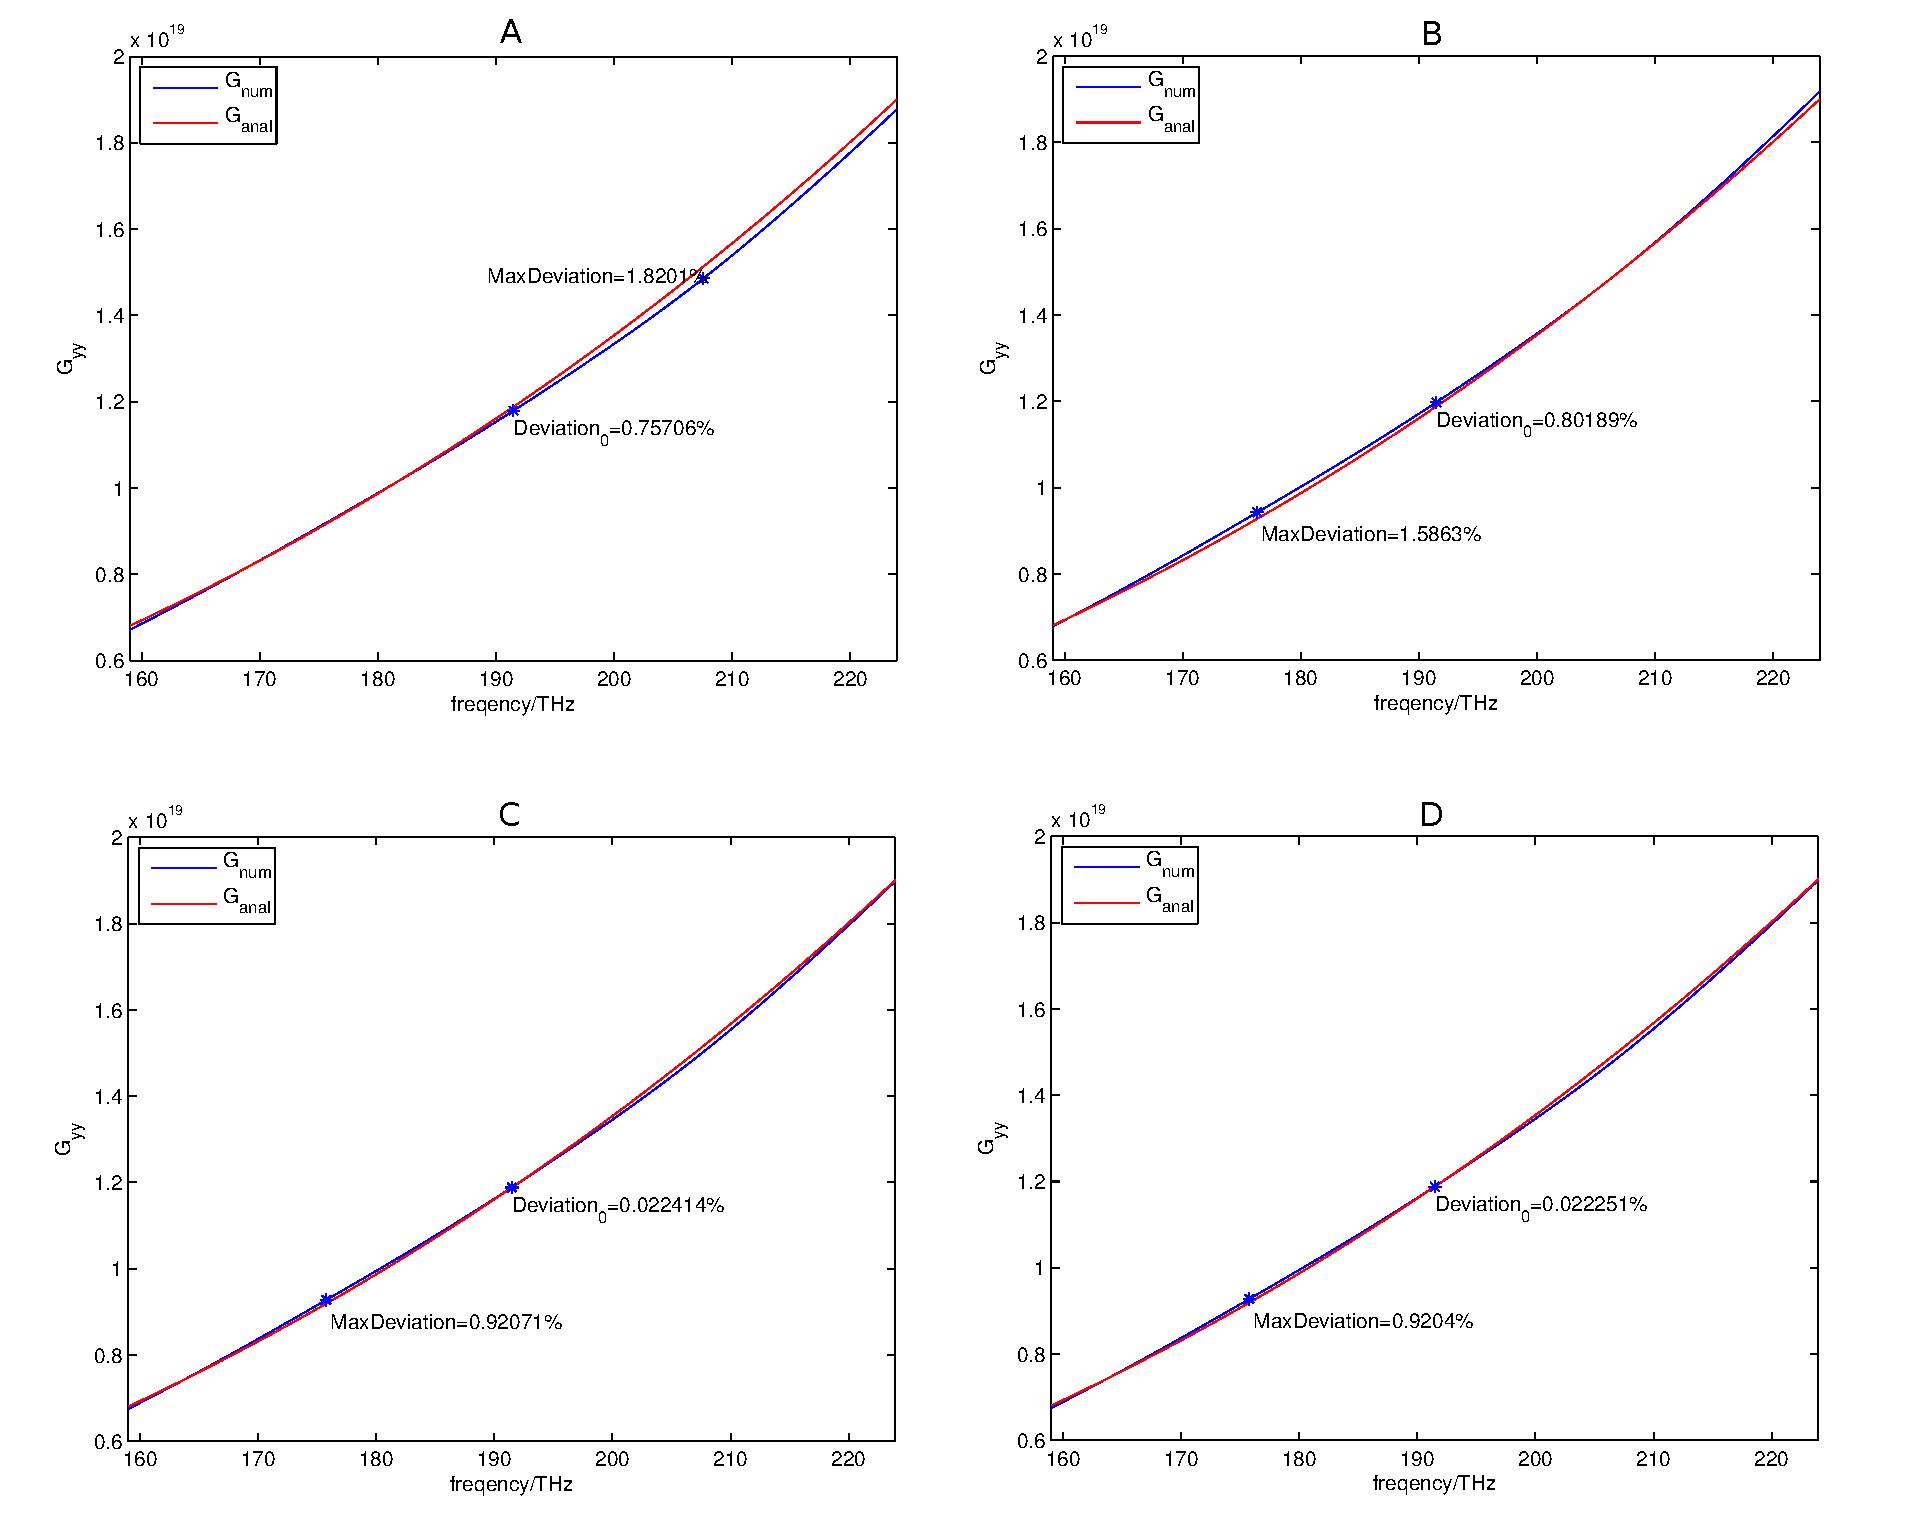
\includegraphics[width=16cm]{./Figs/Ghom_11_12_13}}
\end{center}
\caption[Comparison of $G_{num}$ with $G_{A}$ in homogeneous medium, in method 1.]{\textbf{Comparison of $G_{num}$ with $G_{A}$ in homogeneous medium with ``none'' interpolation setting. (A-C) used many-joint-monitor approach, (D) used shifting-meshing-zone approach. (A)}: the $\mathbf{G}^{Num}$ curve is obtained from the monitor placed at (10, 0, 0) nm. The two deviation values given in every subplot are the maximum deviation in the interested frequency range and the deviation at the dipole source's peak frequency, respectively. \textbf{(B)}: the $\mathbf{G}^{Num}$ curve is obtained from the monitor placed at (-10, 0, 0) nm. \textbf{(C)}: the $\mathbf{G}^{Num}$ curve is obtained by averaging the data of the two monitors in (A) and (B). \textbf{(D)}: the $\mathbf{G}^{Num}$ curve is obtained by shifting the meshing zone with +10 nm in x-axis direction, with the dipole source and time monitor coordinating at the origin.}
\label{Ghom_11_12_13}
\end{figure}
By averaging the two values obtained from the two monitors, we finally find the center frequency deviation as small as 0.022\% (Fig.\ref{Ghom_11_12_13} (C)).


Another calculation approach is moving the FDTD mesh zone. In this case, we shift the FDTD calculation zone by +10 nm in the x-axis direction, so that the monitors are on the meshing grid points. We call this setting the shifting-meshing-zone approach. It gives almost the same result as the approach above. (Fig.\ref{Ghom_11_12_13} (D)).


Alternatively, we can make the interpolation to the ``nearest mesh cell'' in Lumerical. If we use the many-joint-monitor approach, in this case, we do not need to set the monitor exactly at the half way of the mesh grid; instead, they can be whatever places close to the interested point. Or, we can move the mesh zone to a distance less than or equal to the half length of mesh grid in x-axis. They can give the exact same results as we have shown in Fig.~\ref{Ghom_11_12_13}.

In contrast, let's place both the dipole source and a time monitor at the origin without shifting the meshing zone. If we set the interpolation method to be either ``none'' or ``nearest mesh cell'' in Lumerical, the maximum deviation in our interested frequency range and at the center frequency increases considerably (Fig.\ref{Ghom_7_14}). And as expected, they are all equivalent to the case that the monitor is at (-10, 0, 0) with ``none'' interpolation in Lumerical (see Fig.\ref{Ghom_11_12_13} (B)).
\begin{figure}[htp]
\centering
\begin{center}
{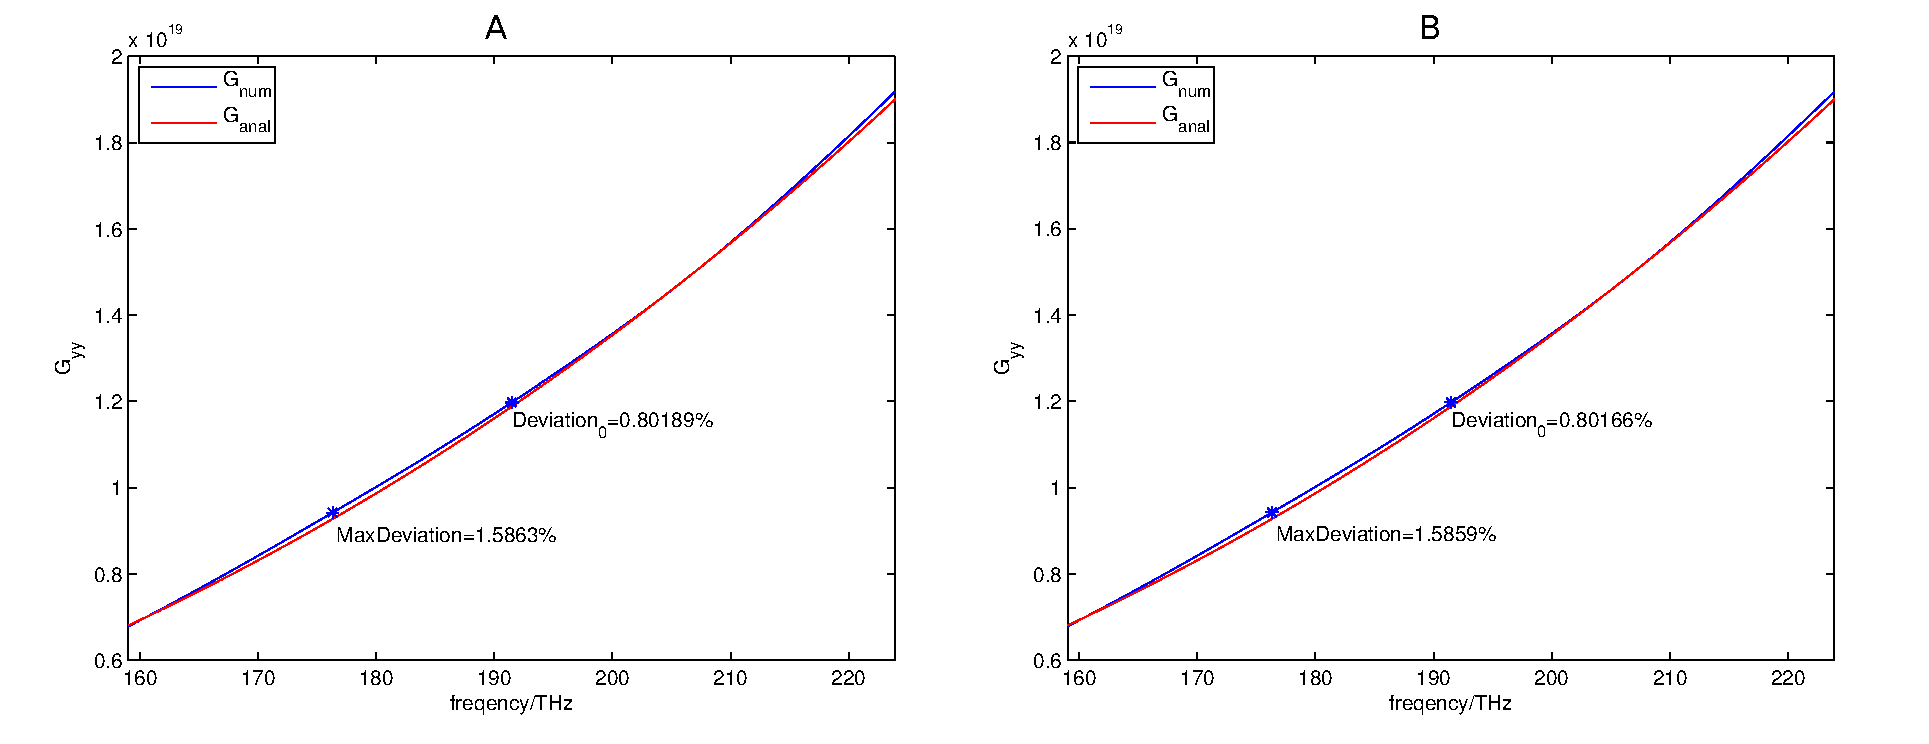
\includegraphics[width=16cm]{./Figs/Ghom_7_14}}
\end{center}
\caption[Comparison of $G_{num}$ with $G^{A}$ in homogeneous medium, in method 2.]{\textbf{Comparison of $G^{num}$ with $G^{A}$ in homogeneous medium with one time monitor and static mesh zone. (A)} Interpolation method is set to ``none'' in Lumerical. \textbf{(B)} Interpolation method is set to ``nearest mesh cell'' in Lumerical. }
\label{Ghom_7_14}
\end{figure}

Based on the discussion above, we can use either the ``many-joint-monitor'' or ``shifting-meshing-zone'' approach to get the exact numerical GFT based on FDTD method. Not only for time monitors, the results above apply to the frequency monitors cases as well. The difference is that, for frequency monitors, there is a ``specified position'' option for interpolation setting, and this option can generate exact interpolated FDTD data at the Yee cell central point. So, ``specified position'' option is preferably used for frequency monitors to reduce the calculation burden and improve the computational accuracy.

In actual 3-D simulation, in order to get the full components of GFT, the many-joint-monitor approach consumes more computer memory for FDTD calculation (every calculation point with 6 time monitors), and the shifting-meshing-zone approach requires parallel runs for three times with three shifts in every parallel run, and generates more data. However, as we have confirmed, the calculation errors are very small; and the improvement on computational accuracy with a good interpolation method is limited. Therefore, for the discussion below, we only use one monitor exactly on the interested point to get the calculation result, in order to save the simulation time and memory.




\subsection{Improve the Accuracy of $G^{A}$ Calculation}

Now, let's briefly introduce some findings on the course of calculating $G^{A}$. I used PC and Micropillar cavity configurations, and verified the analytical GFs with the numerical ones. The final results are plotted in Section~\ref{section:verifyGAGN}. $G^{A}$ agrees very well with $G^{num}$, using my final approach. To improve the accuracy of analytical GFs calculations, one needs to consider how to improve the performance of mode monitoring. One factor that may contribute to the performance is the PML boundary conditions, which determine if the finite simulation zone can give a light-propagating condition close to the real cavity with a large area. I find that by changing the PML in a small range, the result may be slightly improved; but to improve the calculation accuracy dramatically, one may need to increase the memory cost and CPU time cost exponentially. Therefore, it is not worth improving the PML settings for our calculation samples.

Now, we turn to other factors. Let us concentrate on the PC cavity's case, and use the ``getdata'' command extracting the full space index and frequency monitor's data from FDTD simulation package. According to my calculation and comparison on different cases, some of the concerns are as follows.

1. The decay rate defined by Harminv is a half of FWHM, which may be different from the definition in other publications on decay rate. Using different definitions of decay rate in GF calculation may result in a wrong wave envelope of GF.

2. The center frequency obtained from Harminv is usually slightly different from actual value from well performed Fourier transformation. For example, for our PC
cavity's case, the center frequency should approximately be $191.4885$ THz, while Harminv gives $191.487$ THz. The frequency shift effect to $G^{A}$ is shown in Fig.~\ref{Gpc_errors}. This may be a result of limited accuracy in Harminv calculation or the fast calculation algorithm of Harminv. So it's better to identify the mode frequency through a long-time FDTD simulation using a time monitor before analytical GF calculations.
\begin{figure}[htp]
\centering
\begin{center}
{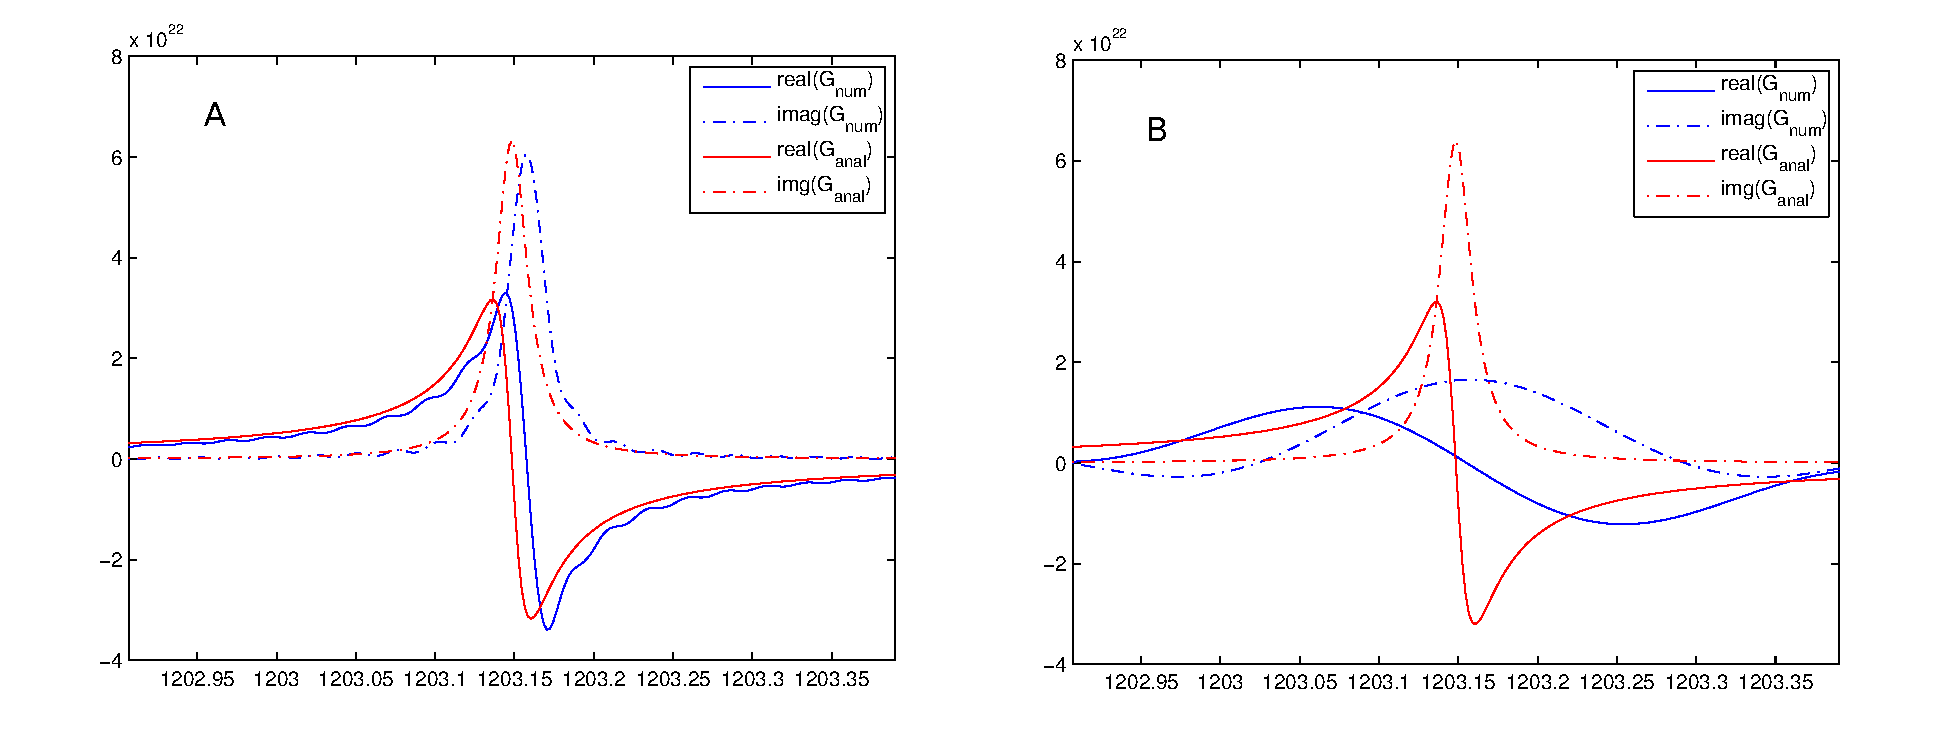
\includegraphics[width=14cm]{./Figs/Gpc_errors}}
\end{center}
\caption[Common problems in calculation.]{\textbf{Common problems in FDTD simulation and GFT calculation. (A)} Frequency shift effect. Using the center frequency of $\omega_0$ from Harminv to calculate $G^{A}$ may result in a frequency shift. Here, Harminv gives $f_0=191.487$ THz, while the exact value from FFT of a long time simulation package is 191.4885 THz. \textbf{(B)} If simulation time is limited, the envelope of $G^{num}$ may be broadened with visible oscillations in a large range (even out of the plotted frequency range). The simulated evolution time $t=25000$ fs for (B); ten times longer for the optimized result in (A). The x-axis is the frequency in unit of $10^{13}$ Hz; y-axis gives the amplitude of GF in an arbitrary unit.}
\label{Gpc_errors}
\end{figure}

3. Limited simulation time will broaden the envelope of $G_{num}$, while the decay rate and related parameters obtained through Harminv could still be credible to get a good $G^{A}$ (see Fig.\ref{Gpc_errors} (B)).

\subsection{Calculations Employing Symmetry}
In practice, we may need to use symmetric boundary settings to improve simulation efficiency. So, it is essential to find the right way to process the data for GF calculation from a symmetric FDTD simulation. Using a ``lum2mat'' command, one can get the reduced data package generated from a symmetric simulation. The size of the reduced data package is usually $1/2$, $1/4$ or $1/8$ of the full simulation. The ``getdata'' command can be used to extract the full size data from a symmetric simulation. With a symmetric simulation, there are at least three ways to handle the data: one is to use ``getdata'' command lines in Lumerical to extract the full space data, and calculate the GFs thereafter; the second approach is to extract the full space data using Matlab code when one calculates GFT in Matlab; and use some tricks in calculation to get the right answer using the reduced data package obtained directly by ``lum2mat'' from *.fsp file.

The first approach is very direct, but will occupy more hard drive space. It is not a good approach if we have a lot of simulation packages to store simultaneously. And the ``getdata'' command normalizes the original data to the signal. The second approach is equivalent to the first approach, but without bringing in unnecessary normalization. The third approach seems to be better than the former ones, because it requires less hard drive space and can be widely used.

We will discuss the third approach now. Borrowed from solid state physics, the conception of ``unit cell'' may be helpful for our discussion. A unit cell is the basic symmetric unit of simulated zone in Lumerical, which is $\frac{1}{2^n}$ of the whole simulation space, where $n$ is the symmetry index. For example, if we do not use a symmetric setting in Lumerical, $n=0$; if we solely use a symmetric setting in $x$-axis, $n=1$; if we set the symmetric condition in both $x$- and $y$-axis, $n=2$.

A unit cell contains several parts according to how they are shared with other units. Take the case of $n=3$ for example (Fig.~\ref{cube}). A unit cell (in color) is in the first quadrant of the 3D space. It contains one element volume $V_0$ (in light blue) isolated to the other cells; it has three shared faces $f_i, \, i=1,2,3$ neighboring to another one unit cell; it also has three shared lines $l_j,\, j=1,2,3$ neighboring with four other units around them; and it has one shared point, the origin point, $p_0$, neighboring with eight other units in the whole coordinate. Notice that the width or height of the shared lines and faces is determined by the gridding or interpolating distance. For instance, the height of $l1$ in $z$-direction is the minimum distance between two gridding points in $z$-direction; a similar rule applies to the width of $l1$ in $y$-direction. As has been observed, a calculation without considering the shared points usually has a large error.
\begin{figure}[htp]
\centering
\begin{center}
{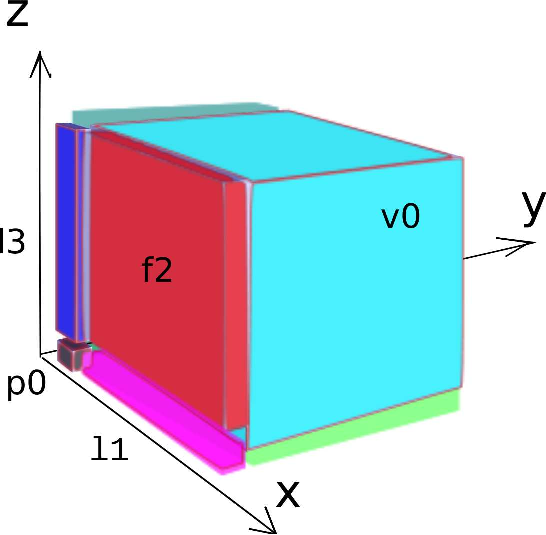
\includegraphics[width=5cm]{./Figs/cube1}}
\end{center}
\caption[Diagram of unit cell cube in the first quadrant.]{\textbf{Diagram of unit cell cube in the first quadrant, when $n=3$.} $V_0$ is the inner cube sharing nothing with other units. $p_0$ is the origin point shared by all 8 units around it. $l_1$ and $l3$ are the line borders in x- and z-axis shared by neighboring 4 units. $f2$ is the face bound in x-z plane shared with 1 neighboring unit.}
\label{cube}
\end{figure}

According to Equ.\eqref{Veff}, if our ``integral'' is only operated over the first quadrant, the effective mode volume should be 8 times the effective mode volume $V_{eff0}$ in the first quadrant. If considering the shared faces, lines and point in the origin, we have
\begin{equation}
 V_{eff0}=V_{v0}+\frac{1}{4}(V_{f1}+V_{f2}+V_{f3})+\frac{1}{2}(V_{l1}+V_{l2}+V_{l3})+\frac{1}{8}V_{p0},
\end{equation}
where we have defined
\begin{subequations}
 \begin{align}
  V_{v0} &=V(2:end,2:end,2:end), \\
  V_{p0} &=V(1,1,1), \\
  V_{l1} &=V(2:end,1,1)=V(:,1,1)-V_0, \\
  V_{l2} &=V(1,2:end,1)=V(1,:,1)-V_0, \\
  V_{l3} &=V(1,1,2:end)=V(1,1,:)-V_0, \\
  V_{f1} &=V(1,2:end,2:end)=V(1,:,:)-Vl2-Vl3-Vs0, \\
  V_{f2} &=V(2:end,1,2:end)=V(:,1,:)-Vl1-Vl3-Vs0, \\
  V_{f3} &=V(2:end,2:end,1)=V(:,:,1)-Vl1-Vl2-Vs0,
 \end{align}
\label{vparts}
\end{subequations}
and $V$ is the matrix form of Equ.\eqref{Veff} in Matlab. Every entry of $V$ above corresponds to the discrete index of the 3-D coordinate of space position. $V$ stores the position data on the meshed grids.


Notice that, according to the manual of Lumerical software, if we use anti-symmetric conditions in one direction--in y-axis, for example--then the E-field values in the plane perpendicular to y-axis will become zero. That is $Ex(:,1,:)=0$ and $Ez(:,1,:)=0$.

On the borders, the variables vary dramatically. And the measured field values (referenced to the Yee cell frame) are not bound to be the values at given coordinate points. So, it is necessary to interpolate the field value into a real coordinate system. And the accuracy of interpolation in the borders determines the total accuracy, considerably.

Now we verify our calculation method introduced above by simulating the PC cavity mode with ``none'' interpolation in Lumerical (``nearest mesh cell'' interpolation setting gives similar results, but we should be more careful to deal with the interpolation in Matlab). Through interpolation, we move the measured field components to the real coordinate points, and refine the mesh grid by $m$ times, which gives the interpolation steps $dx_{interp}=dx/m, \,dy_{interp}=dy/m$ and $dz_{interp}=dz/m$. Without the interpolation, the measured field values have actually been  shifted a half length of the edges of the Yee cell in some direction. The calculated GFs with different interpolation settings are shown in Fig.~\ref{G68_interp}, where subfigure ($A$) gives the standard values for comparisons.
\begin{figure}[htp]
\centering
\begin{center}
{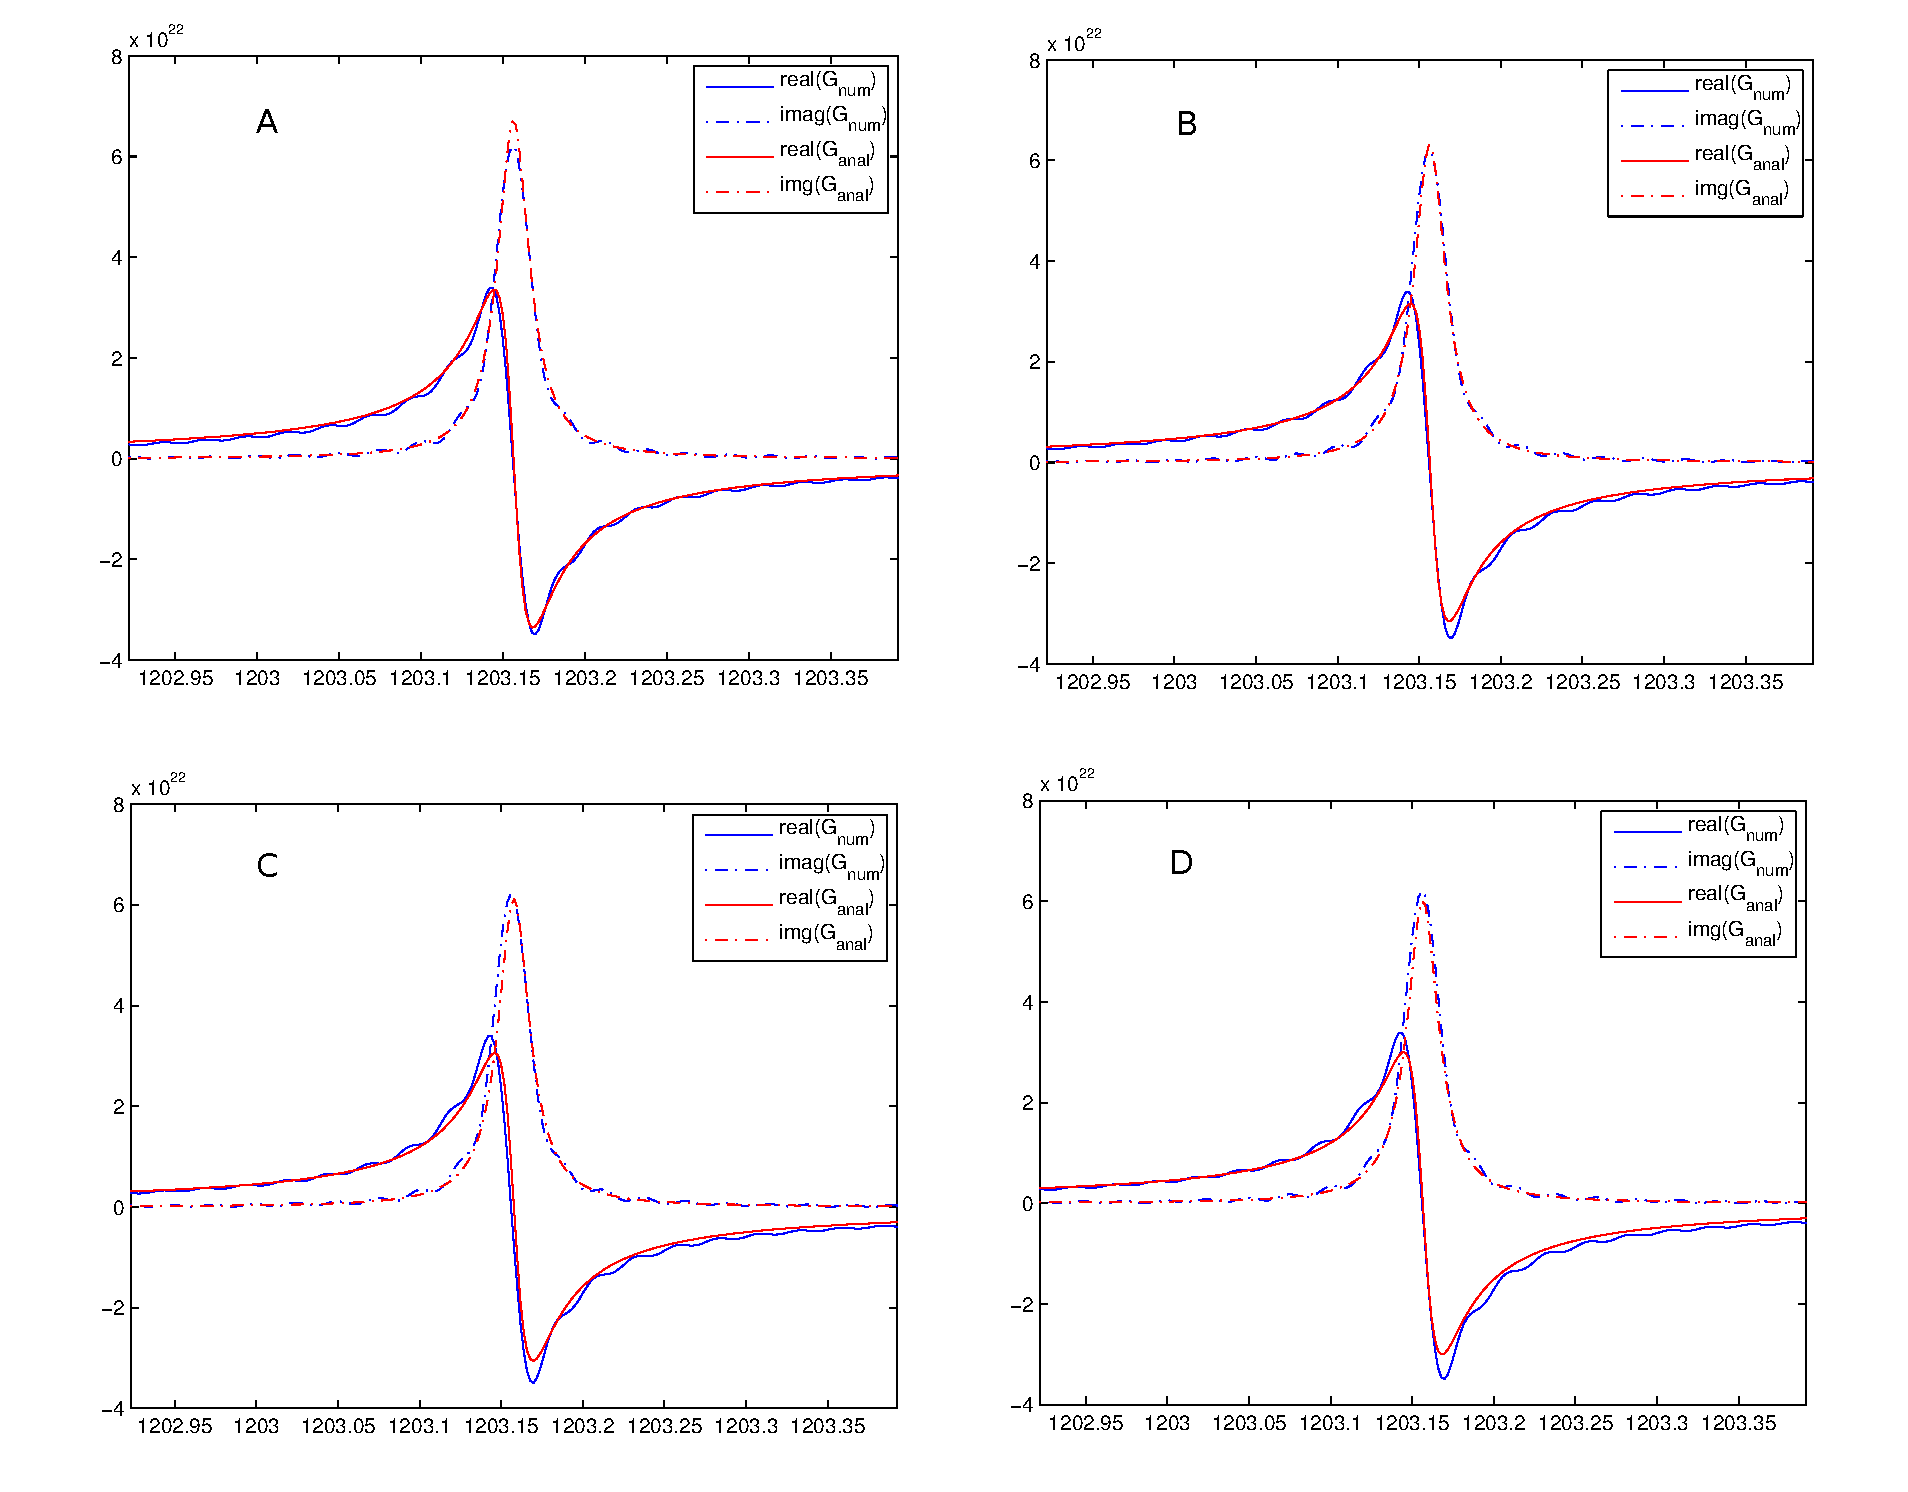
\includegraphics[width=16cm]{./Figs/G68_interp}}
\end{center}
\caption[Comparison of GF with different interpolation parameters.]{\textbf{Comparison of GF with different interpolation parameters with $n=3$ symmetric condition settings.} In the calculation, I used $191.4883$ THz as the mode resonance. The decay rate is read from Harminv. \textbf{(A)} No interpolation, and used full space data. $V_{eff} = 6.3556e^{-20}m^{-3},\, V_{eff0} = 9.2952e^{-21}m^{-3}$. \textbf{(B)} Interpolated with $m=1$, and used reduced data. $V_{eff} =  6.7144e^{-20}m^{-3},\,V_{eff0} = 8.3930e^{-21}m^{-3}$. \textbf{(C)} Interpolated with $m=2$, and used reduced data. $V_{eff} =  6.9317e^{-20}m^{-3},\, V_{eff0} = 8.6646e^{-21}m^{-3}$. \textbf{(D)} Interpolated with $m=4$, and used reduced data. $V_{eff} =  7.0529e^{-20}m^{-3},\, V_{eff0} =  8.8161e^{-21}m^{-3}$. The x-axis is the frequency in unit of $10^{13}$ Hz; y-axis gives the amplitude of GF in an arbitrary unit.}
\label{G68_interp}
\end{figure}
It turns out the interpolation with higher $m$ will produce more deviation (with reduced amplitude with larger $V_{eff}$, a frequency shift to the high-frequency end). This may be caused by the non-matching of Yee cell measured points with our expected measured points.

Limited by the time, I leave the test on interpolations with ``specified position'', optimized ``PML'' and other improved settings in Lumerical as an open research question.

\subsection{Summary}
Through the discussions above, I have verified the analytical and numerical GFs are equivalent, with acceptable deviations ($\leq 2\%$ or so). I proved that we need to run the simulation long enough to get a credible $G^{num}$, and need to adjust the resonance produced by Harminv in order to avoid the resonance shifting effect in $G^{A}$. Some trials on improving the calculation performance are discussed as well, but the accuracy level with our present settings is already high enough. Similarly, more discussions on simulation with symmetric settings and other factors should be carried on if they cause considerable errors in specific cases.
